%==============================================================================
% COM 837 - ML for Wireless Communication Systems
% Assignment 2 - Single consolidated report
%
% Build:  pdflatex report.tex   (run twice so references resolve)
% Figures are expected in ./figures/
%==============================================================================
\documentclass[11pt,a4paper]{article}

\usepackage[margin=1in]{geometry}
\usepackage{amsmath,amssymb}
\usepackage{booktabs}
\usepackage{graphicx}
\usepackage{float}
\usepackage{caption}
\usepackage{fancyhdr}
\usepackage{microtype}
\usepackage{parskip}
\usepackage[hidelinks]{hyperref}

\captionsetup{font=small,labelfont=bf}

\pagestyle{fancy}
\fancyhf{}
\lhead{\small ML for Wireless Communication}
\rhead{\small Assignment 2}
\cfoot{\thepage}
\renewcommand{\headrulewidth}{0.4pt}

\setlength{\headheight}{14pt}

\title{\vspace{-1.5cm}\textbf{Assignment 2}\\[0.3em]
       \large COM 837 --- ML for Wireless Communication Systems}
\author{Taral (IMT2023588)}
\date{}

\begin{document}

\maketitle
\thispagestyle{fancy}

\noindent
All results in this report are produced by the scripts in the accompanying GitHub
repository. The Question~1 dataset is generated by the provided
\texttt{generate\_dataset.py}, used without modification. The Question~2 dataset is
generated by \texttt{generate\_qam\_dataset.py} with random seed 67. All random seeds are
fixed (\texttt{random\_state = 42} for the train/test splits and for K-means), so every
number and figure below is reproducible by re-running the code.

%==============================================================================
\section{SVM for LOS/NLOS Identification}
%==============================================================================

\subsection{Feature Extraction}

Each row of the dataset is one channel realisation described by six complex taps and their
delays. The tap amplitudes and powers are

\begin{equation}
|h_l| = \sqrt{h_{\mathrm{real},l}^2 + h_{\mathrm{imag},l}^2},
\qquad
P_l = |h_l|^2, \qquad l = 0,\dots,L-1, \quad L = 6 .
\end{equation}

Five scalar features are extracted per realisation, following the definitions of
Huang \emph{et al.} Because each feature is a statistic over the $L = 6$ taps of a single
snapshot, all moments are population statistics (\texttt{ddof} $=0$).

\subsubsection{Kurtosis of the Received Power}

Kurtosis measures the peakedness of the amplitude distribution across taps:

\begin{equation}
\mathcal{K} = \frac{\mathbb{E}\!\left[\left(|h| - \mu_{|h|}\right)^4\right]}{\sigma_{|h|}^4},
\end{equation}

where $\mu_{|h|}$ and $\sigma_{|h|}$ are the mean and standard deviation of the tap
amplitudes. In a LOS snapshot one dominant tap sits far out in the tail of the amplitude
distribution, which makes the distribution peaked and raises the kurtosis. NLOS amplitudes
are comparatively flat.

\subsubsection{Skewness of the Received Power}

Skewness measures the asymmetry of the same distribution:

\begin{equation}
\mathcal{S} = \frac{\mathbb{E}\!\left[\left(|h| - \mu_{|h|}\right)^3\right]}{\sigma_{|h|}^3}.
\end{equation}

A Rayleigh (NLOS) amplitude distribution and a Rician (LOS) one differ in asymmetry, so
this carries LOS/NLOS information independent of the peakedness.

\subsubsection{Rising Time}

The rising time is the delay gap between the first arriving path and the strongest path:

\begin{equation}
\Delta\tau = \tau\!\left(\arg\max_l |h_l|\right) - \min_l \tau_l .
\end{equation}

In LOS the first path is also the strongest, so $\Delta\tau$ collapses to $0$~ns. In NLOS
the first path may be attenuated by blockage or diffraction and the strongest path arrives
later, giving a larger value.

\subsubsection{Root Mean Square Delay Spread}

The power-weighted mean excess delay and the RMS delay spread are

\begin{equation}
\tau_m = \frac{\sum_{l} \tau_l P_l}{\sum_{l} P_l},
\qquad
\tau_{\mathrm{rms}} = \sqrt{\frac{\sum_{l} (\tau_l - \tau_m)^2 P_l}{\sum_{l} P_l}} .
\end{equation}

NLOS power is spread across many comparable taps at long delays, so $\tau_{\mathrm{rms}}$
is large; LOS power is concentrated on the first tap, so it is small. Units are nanoseconds.

\subsubsection{Rician $K$-Factor}

The $K$-factor is implemented exactly as given in the reference paper,

\begin{equation}
K_r = \frac{|h|^2_{\max}}{2\,\sigma^2_{|h|}},
\label{eq:kfactor}
\end{equation}

i.e. the dominant tap power normalised by the \emph{variance} of the tap amplitudes. This
choice has a consequence that is examined in Section~\ref{sec:kdiscussion}.

\subsubsection{Sanity Check on the Extracted Features}

Table~\ref{tab:featuremeans} lists the class-conditional means at the highest SNR, where the
features are least corrupted by noise.

\begin{table}[H]
\centering
\caption{Class-conditional feature means at SNR $=30$~dB.}
\label{tab:featuremeans}
\begin{tabular}{lrr}
\toprule
Feature & NLOS ($-1$) & LOS ($+1$) \\
\midrule
Kurtosis                    & 2.16  & 3.87 \\
Skewness                    & 0.35  & 1.61 \\
Rising time (ns)            & 28.15 & 0.00 \\
RMS delay spread (ns)       & 45.19 & 6.98 \\
Rician $K$-factor, Eq.~\eqref{eq:kfactor} & 6.56 & 4.58 \\
\bottomrule
\end{tabular}
\end{table}

Four of the five features order themselves exactly as the physical reasoning predicts. The
LOS snapshots are more peaked and more skewed, their strongest tap is their first tap so the
rising time is identically zero, and their power is concentrated at short delay so the RMS
delay spread is roughly $6.5\times$ smaller than NLOS. The $K$-factor of
Eq.~\eqref{eq:kfactor} is the exception: it comes out \emph{lower} for LOS than for NLOS.
This is not an implementation error and is explained in Section~\ref{sec:kdiscussion}.

%------------------------------------------------------------------------------
\subsection{Per-Feature and Combined SVM Classification}
%------------------------------------------------------------------------------

\subsubsection{Experimental Setup}

Six classifiers are trained independently at each SNR: SVM-1 to SVM-5 use one feature each,
and SVM-6 uses all five. At every SNR the data are split 80/20 with stratification on the
label, a \texttt{StandardScaler} is fitted on the training set only and applied to the test
set, and an RBF-kernel SVM with $C = 1$ is trained. The same split is shared by all six
classifiers at a given SNR so their accuracies are directly comparable.

\subsubsection{Classification Results}

\begin{table}[H]
\centering
\caption{LOS/NLOS classification accuracy (\%) for the six SVM classifiers.}
\label{tab:q1b}
\begin{tabular}{crrrrrr}
\toprule
SNR (dB) & Kurtosis & Skewness & Rise time & RMS delay & Rician $K$ & All five \\
\midrule
 0 & 59.50 & 58.75 & 79.75 & 88.50 & 60.00 & \textbf{89.25} \\
 5 & 82.25 & 84.50 & 83.00 & 90.00 & 68.00 & \textbf{98.25} \\
10 & 90.75 & 93.50 & 81.25 & 93.00 & 76.00 & \textbf{99.50} \\
15 & 93.25 & 95.00 & 83.00 & 97.25 & 81.75 & \textbf{99.75} \\
20 & 93.75 & 94.50 & 83.00 & 98.25 & 81.75 & \textbf{100.00} \\
25 & 93.50 & 93.75 & 82.50 & 98.25 & 82.50 & \textbf{100.00} \\
30 & 93.75 & 95.50 & 82.50 & 98.75 & 81.50 & \textbf{100.00} \\
\bottomrule
\end{tabular}
\end{table}

\begin{figure}[H]
\centering
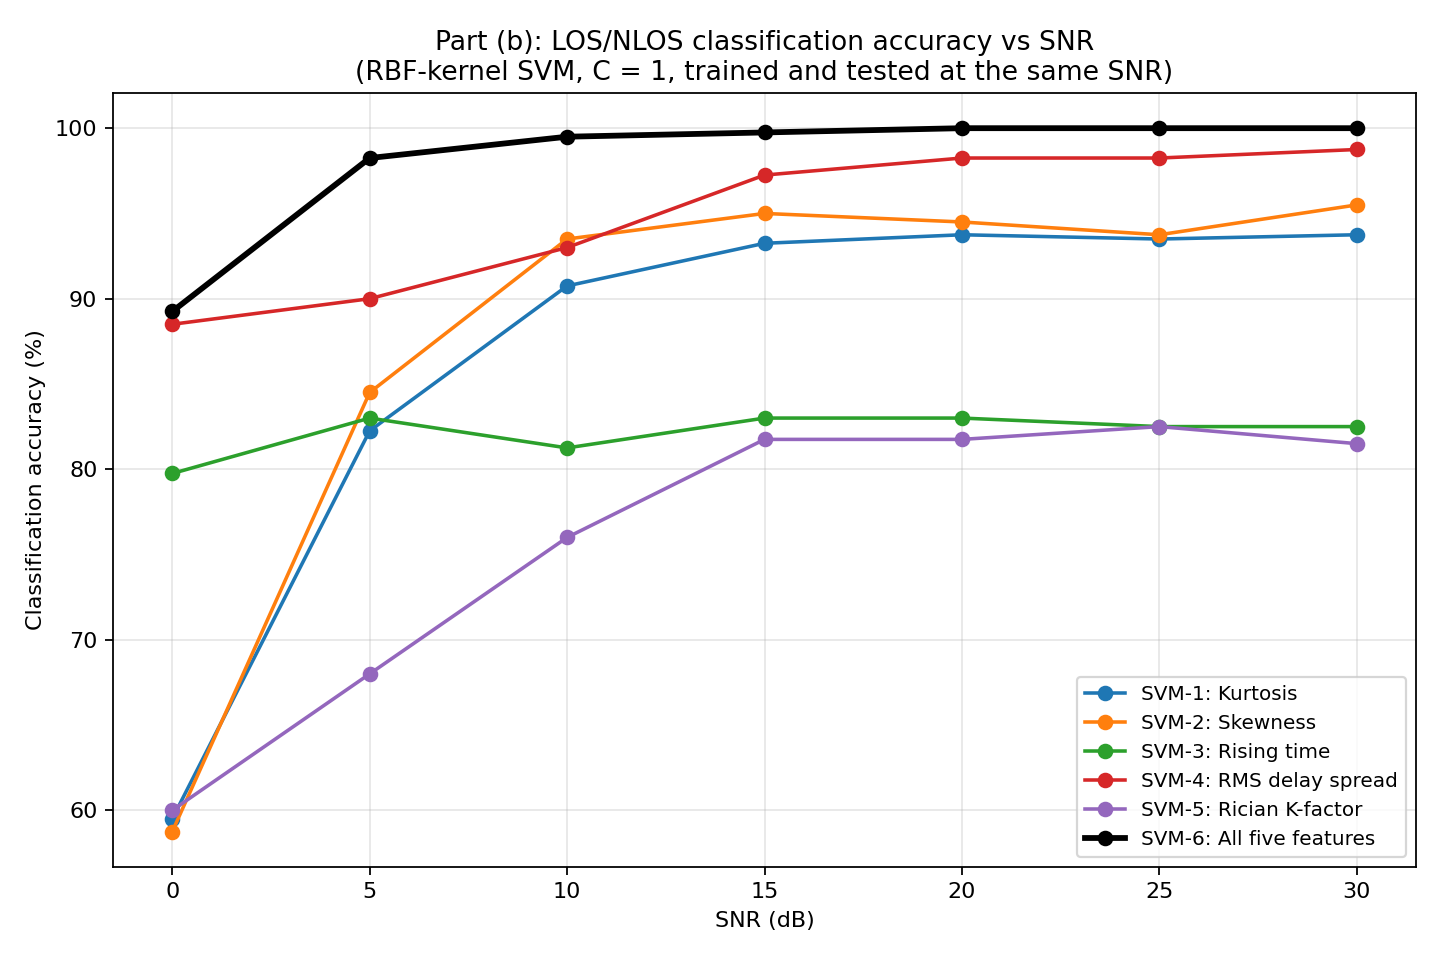
\includegraphics[width=0.88\textwidth]{figures/partb_accuracy_vs_snr.png}
\caption{Classification accuracy versus SNR for the six SVM classifiers. The combined
five-feature classifier (black) dominates every single-feature classifier at every SNR.}
\label{fig:q1b}
\end{figure}

\subsubsection{Discussion}

\paragraph{Which single feature performs best overall, and why?}
The RMS delay spread (SVM-4). It is the best single feature at every SNR, from 88.50\% at
0~dB to 98.75\% at 30~dB, and it is the only one that stays above 88\% across the whole
range.

The reason lies in the channel model. The two classes are generated with different delay
statistics: LOS delays are drawn from an exponential distribution of mean 30~ns with a
matching 30~ns power decay constant, whereas NLOS uses 100~ns for both. The two classes
therefore differ not only in how power is distributed over the taps but in the span of
delays over which those taps are placed. The RMS delay spread measures exactly the second
central moment of the power delay profile, and it is fed by both effects simultaneously: the
delay axis is stretched by roughly $3.3\times$ in NLOS, and the power weighting is spread
across all six taps instead of being concentrated on tap~0. The resulting class means at
30~dB are 45.19~ns against 6.98~ns.

By contrast, kurtosis, skewness and the $K$-factor use only the amplitude distribution and
discard the delay axis entirely. They estimate a shape statistic from six samples, which is
inherently high-variance, and they saturate in the 82--95\% range.

\paragraph{Does combining all five features improve on the best single feature, and where is
the improvement most noticeable?}
Yes, at every SNR. The margin of SVM-6 over the best single feature is:

\begin{table}[H]
\centering
\caption{Accuracy gain (percentage points) of SVM-6 over the best single-feature classifier.}
\label{tab:q1gain}
\begin{tabular}{crrrrrrr}
\toprule
SNR (dB) & 0 & 5 & 10 & 15 & 20 & 25 & 30 \\
\midrule
Gain (pp) & $+0.75$ & $\mathbf{+8.25}$ & $\mathbf{+6.50}$ & $+2.50$ & $+1.75$ & $+1.75$ & $+1.25$ \\
\bottomrule
\end{tabular}
\end{table}

The improvement is most noticeable at 5~dB and 10~dB. That is the transition region: the
delay-domain feature is already partly informative there, and the amplitude-domain features
have just become usable, with kurtosis and skewness jumping from roughly 59\% at 0~dB to
82--93\% at 5--10~dB. Because the two families of features make different kinds of mistakes,
one reading delay geometry and the other reading amplitude statistics, their errors are only
weakly correlated and the RBF kernel can find a boundary in five dimensions that neither can
find in one.

At the two extremes the gain shrinks, for opposite reasons. At 0~dB the other four features
are close to useless, between 58\% and 80\%, so they contribute almost nothing to
$\tau_{\mathrm{rms}}$ and the gain is only 0.75~pp. At 20~dB and above the delay spread
alone is already at 98\%, leaving very little headroom, although the combination does reach a
clean 100\%.

\paragraph{Which feature performs poorly at low SNR despite being physically meaningful?}
\label{sec:kdiscussion}
The Rician $K$-factor. It is the most physically direct statement of whether a dominant path
is present, and it is the quantity on which classical threshold-based LOS identification has
historically been built, yet it achieves only 60.00\% at 0~dB and is the weakest feature
overall. Two distinct mechanisms are responsible.

\emph{(i) The low-SNR failure: noise floods the weak taps.} The generator adds AWGN of
variance $1/(L\cdot\mathrm{SNR})$ per tap. At 0~dB this is $1/6 \approx 0.167$ per tap
against a total clean channel power of 1. In a LOS realisation, taps 1--5 collectively carry
only $1/(K+1) \approx 0.11$ of the power, roughly $0.02$ per tap, so the noise is about eight
times stronger than the scattered taps it sits on. Those taps stop reporting the channel and
start reporting the noise floor, and a noisy LOS snapshot begins to look like a noisy NLOS
one. Table~\ref{tab:drift} makes this explicit: as the SNR falls, the LOS statistics collapse
towards the NLOS ones, while the NLOS statistics barely move, because NLOS taps are all of
comparable size and are far less distorted by an added noise floor.

\begin{table}[H]
\centering
\caption{Feature drift with SNR, shown as LOS mean $\rightarrow$ NLOS mean.}
\label{tab:drift}
\begin{tabular}{lccc}
\toprule
Feature & 30 dB & 10 dB & 0 dB \\
\midrule
Kurtosis                    & $3.87 \rightarrow 2.16$ & $3.73 \rightarrow 2.19$ & $\mathbf{2.55 \rightarrow 2.17}$ \\
Skewness                    & $1.61 \rightarrow 0.35$ & $1.53 \rightarrow 0.39$ & $\mathbf{0.69 \rightarrow 0.30}$ \\
Rician $K$, Eq.~\eqref{eq:kfactor} & $4.58 \rightarrow 6.56$ & $5.06 \rightarrow 7.09$ & $\mathbf{6.97 \rightarrow 8.10}$ \\
RMS delay spread (ns)       & $6.98 \rightarrow 45.19$ & $11.91 \rightarrow 51.89$ & $20.47 \rightarrow 65.37$ \\
\bottomrule
\end{tabular}
\end{table}

Kurtosis, skewness and the $K$-factor all converge to nearly identical class means at 0~dB,
which is why all three sit at 58--60\% accuracy there. The RMS delay spread is the outlier
that survives, because its separation is anchored in the delay axis and the $\tau$ columns
are noiseless.

\emph{(ii) An additional, SNR-independent problem with Eq.~\eqref{eq:kfactor}.} That equation
normalises the peak power by the variance of the tap \emph{amplitudes}. With only $L = 6$
taps and one dominant tap of amplitude $a$, the dominant tap inflates the denominator as much
as the numerator: $\sigma^2_{|h|} \approx a^2 (L-1)/L^2$, so

\begin{equation}
K_r \approx \frac{L^2}{2(L-1)} = 3.6
\end{equation}

regardless of how strong the LOS component actually is. The estimator saturates. This is why
the LOS mean (4.58) falls below the NLOS mean (6.56) in Table~\ref{tab:featuremeans}, and why
the feature plateaus near 82\% even at 30~dB.

To confirm that this is a property of the definition rather than of the physics, the same
single-feature experiment was repeated with the textbook form
$K = P_{\mathrm{peak}} / (P_{\mathrm{total}} - P_{\mathrm{peak}})$, which involves no such
cancellation.

\begin{table}[H]
\centering
\caption{Single-feature accuracy (\%) under the two $K$-factor definitions.}
\label{tab:kdefs}
\begin{tabular}{crrrrrrr}
\toprule
SNR (dB) & 0 & 5 & 10 & 15 & 20 & 25 & 30 \\
\midrule
Eq.~\eqref{eq:kfactor}                 & 60.00 & 68.00 & 76.00 & 81.75 & 81.75 & 82.50 & 81.50 \\
$P_{\mathrm{peak}}/P_{\mathrm{residual}}$ & 65.75 & 87.75 & 96.25 & 96.75 & 97.50 & 98.00 & 98.00 \\
\bottomrule
\end{tabular}
\end{table}

Under the standard definition the $K$-factor becomes one of the strongest features at high
SNR, at 98.00\%, while still collapsing to 65.75\% at 0~dB. That is precisely the
``physically meaningful but fails at low SNR'' behaviour the question points at. The main
results in this report retain Eq.~\eqref{eq:kfactor} as specified by the reference paper;
Table~\ref{tab:kdefs} is reported only to separate the two causes.

%------------------------------------------------------------------------------
\subsection{Training Strategy Comparison}
%------------------------------------------------------------------------------

The combined five-feature classifier SVM-6 is trained once on the 25~dB training split and
evaluated on the test split of every SNR. The scaler is frozen along with the classifier: a
deployed receiver would not know the target-SNR statistics, so refitting the scaler per SNR
would leak information the real system cannot have. The matched curve reuses the SVM-6
results of Table~\ref{tab:q1b}, and both curves are evaluated on identical test sets.

\begin{table}[H]
\centering
\caption{Matched-SNR training versus training only at 25~dB, accuracy (\%).}
\label{tab:q1c}
\begin{tabular}{crrr}
\toprule
SNR (dB) & Train $=$ Test SNR & Train at 25 dB & Gap (pp) \\
\midrule
 0 &  89.25 &  58.00 & $\mathbf{-31.25}$ \\
 5 &  98.25 &  78.25 & $\mathbf{-20.00}$ \\
10 &  99.50 &  97.50 & $-2.00$ \\
15 &  99.75 &  99.50 & $-0.25$ \\
20 & 100.00 &  99.75 & $-0.25$ \\
25 & 100.00 & 100.00 & $0.00$ \\
30 & 100.00 & 100.00 & $0.00$ \\
\bottomrule
\end{tabular}
\end{table}

\begin{figure}[H]
\centering
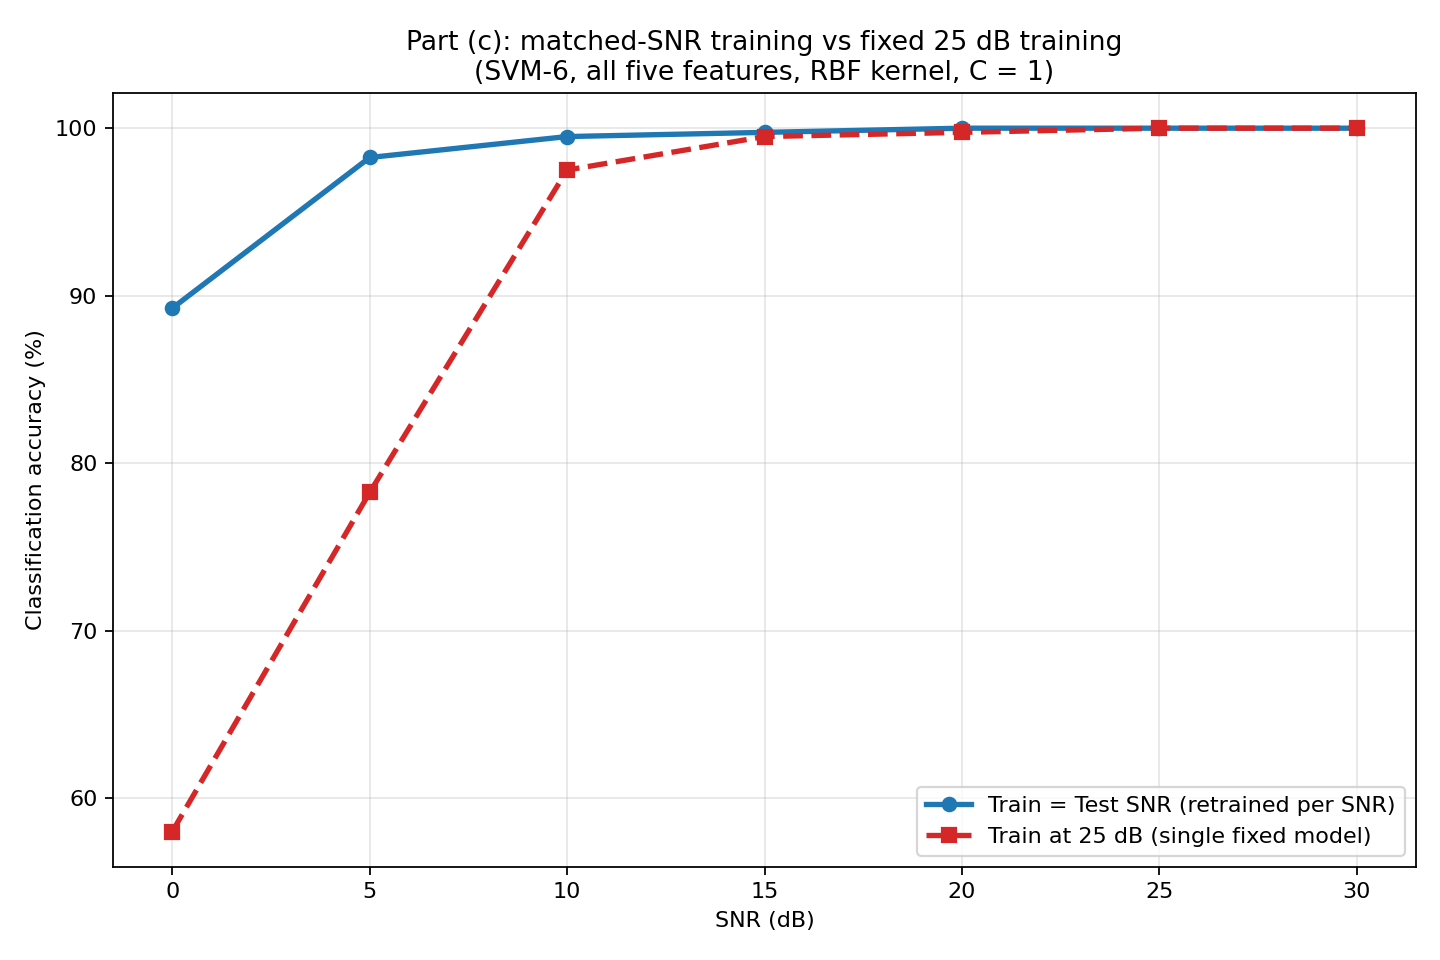
\includegraphics[width=0.85\textwidth]{figures/partc_train25_vs_matched.png}
\caption{Matched-SNR training versus a single model trained only at 25~dB.}
\label{fig:q1c}
\end{figure}

\subsubsection{Discussion}

\paragraph{At high SNR, do the two curves agree?}
Yes. They are identical at 25 and 30~dB and within 0.25~pp at 15 and 20~dB, so the two curves
are indistinguishable above roughly 12~dB.

This shows that the features have become effectively SNR-invariant once the noise floor drops
below the weakest taps. From Table~\ref{tab:drift}, between 15 and 30~dB the LOS kurtosis
moves only from 3.83 to 3.87 and the skewness from 1.59 to 1.61, the rising time is pinned at
zero, and $\tau_{\mathrm{rms}}$ moves from 9.09 to 6.98~ns. The feature distributions have
converged to their noiseless limits, so the same region of feature space is occupied at 25~dB
as at 30~dB. A decision boundary fitted in that region is therefore valid at any other high
SNR, and there is nothing left for retraining to adapt to. In practice this means that above
roughly 15~dB a receiver can train once and deploy without loss.

\paragraph{At low SNR, which strategy performs better, and by how much?}
Matched training, decisively: $+31.25$~pp at 0~dB (89.25\% against 58.00\%) and $+20.00$~pp
at 5~dB (98.25\% against 78.25\%). At 0~dB the fixed model is only 8~pp above a coin flip and
has essentially stopped working.

The cause is covariate shift. The 25~dB model has learned a boundary positioned for tight,
well-separated clusters, with LOS near (kurtosis 3.87, $\tau_{\mathrm{rms}}$ 7.2~ns) and NLOS
near (2.16, 45.5~ns). At 0~dB the LOS cluster has migrated to (2.55, 20.5~ns) and the NLOS
cluster to (2.17, 65.4~ns), so the LOS test points now land where the model's training data
placed NLOS and are confidently misclassified. Two effects compound this. First, the frozen
scaler normalises the 0~dB features by 25~dB statistics, so every feature arrives offset from
where the RBF kernel expects it; because the RBF kernel is local, points far from the training
support fall into a region where the decision function has no meaningful support. Second, the
classes have genuinely moved closer together, and even the matched model only reaches 89.25\%
at 0~dB, so part of the information has been destroyed by noise. A model trained at a single
high SNR has never seen an overlapping pair of classes and has no basis for placing a
conservative boundary.

Stated generally, a classifier trained at one high SNR is implicitly a classifier of noiseless
channel geometry, and it assumes the features it receives are estimates of that geometry. At
low SNR the assumption is violated, because the features then estimate the noise as much as
the channel.

\paragraph{Would training at a low SNR and testing across all SNR give a different result?}
Yes, and the asymmetry is the interesting part.

Reasoning from Table~\ref{tab:drift}: as the SNR rises, noise-corrupted feature values move
monotonically towards their clean values, and they move \emph{inward}. The low-SNR LOS and
NLOS clusters are broad and overlapping, and the high-SNR clusters sit nested inside that
overlap region at its two extremes. A boundary drawn through the middle of the smeared 0~dB
distributions therefore still lands between the two tight high-SNR clusters. It will be
roughly in the right place, merely badly positioned: hedged against noise that is no longer
present, and so not tight enough to exploit the clean separation. The 25~dB $\rightarrow$ 0~dB
direction enjoys no such protection, because the boundary sits at one extreme of the space and
the test points migrate straight past it.

The prediction is therefore that a 0~dB-trained model degrades gracefully rather than
collapsing: it should hold roughly its own 0~dB accuracy across the whole range but never
reach the 100\% that matched training attains at high SNR. Running the experiment confirms
this.

\begin{table}[H]
\centering
\caption{Accuracy (\%) of SVM-6 trained at a single fixed SNR and tested across all SNRs.}
\label{tab:q1c2}
\begin{tabular}{crrrrrrr}
\toprule
Trained at & 0 dB & 5 dB & 10 dB & 15 dB & 20 dB & 25 dB & 30 dB \\
\midrule
 0 dB & 89.25 & 92.25 & 90.00 & 90.50 & 91.25 &  90.75 &  89.75 \\
 5 dB & 80.75 & 98.25 & 98.00 & 97.75 & 98.25 &  97.75 &  97.75 \\
25 dB & 58.00 & 78.25 & 97.50 & 99.50 & 99.75 & 100.00 & 100.00 \\
\bottomrule
\end{tabular}
\end{table}

The 0~dB model is nearly flat at about 90\% everywhere, far more robust than the 25~dB model
but with a hard ceiling. Training at the worst expected SNR buys robustness at the cost of
peak accuracy; training at the best SNR buys peak accuracy at the cost of catastrophic
low-SNR failure. The 5~dB row shows the sensible compromise, holding about 98\% from 5~dB
upward for only an 8.5~pp loss at 0~dB. If a single fixed model must be deployed, it should
be trained near the low end of the operating range rather than the high end, or better still
on data pooled across SNRs.

%==============================================================================
\section{Constellation Demodulation and Clustering using K-Means}
%==============================================================================

\subsection{Dataset Generation}

A square 16-QAM constellation is built with in-phase and quadrature coordinates drawn from
$\{-3,-1,1,3\}$. The raw grid has average symbol energy
$\mathbb{E}[|s|^2] = \mathbb{E}[I^2] + \mathbb{E}[Q^2] = 5 + 5 = 10$, so every point is
divided by $\sqrt{10}$ to force $E_s = 1$:

\begin{equation}
x_I,\, x_Q \in \left\{ \tfrac{-3}{\sqrt{10}},\, \tfrac{-1}{\sqrt{10}},\,
\tfrac{1}{\sqrt{10}},\, \tfrac{3}{\sqrt{10}} \right\}.
\end{equation}

With $E_s = 1$ the total noise power is simply $N_0 = 1/\mathrm{SNR}_{\mathrm{lin}}$, split
equally between the two real dimensions, so each dimension receives variance $N_0/2$. For
each SNR in $\{0,5,10,15,20,25,30\}$~dB, 200 samples are generated per constellation point,
giving 3200 rows per SNR and 22{,}400 rows overall. The random seed is 67.

One reference number is used repeatedly below. After scaling, the nearest-neighbour symbol
spacing is $2/\sqrt{10} = 0.6325$, which should be compared against the per-axis noise
standard deviation in Table~\ref{tab:noise}.

\begin{table}[H]
\centering
\caption{Per-axis noise standard deviation relative to the symbol spacing $0.6325$.}
\label{tab:noise}
\begin{tabular}{crrrrrrr}
\toprule
SNR (dB) & 0 & 5 & 10 & 15 & 20 & 25 & 30 \\
\midrule
$\sigma$ per axis        & 0.707 & 0.398 & 0.224 & 0.126 & 0.071 & 0.040 & 0.022 \\
$\sigma\,/\,$spacing     & \textbf{1.12} & 0.63 & 0.35 & 0.20 & 0.11 & 0.06 & 0.04 \\
\bottomrule
\end{tabular}
\end{table}

At 0~dB the noise standard deviation exceeds the distance between adjacent symbols. That
single fact explains most of what follows.

\subsection{Amplitude and Phase Features}

Two features are appended to every received sample $z = x_I + j x_Q$:

\begin{equation}
r = \sqrt{x_I^2 + x_Q^2},
\qquad
\theta = \operatorname{atan2}(x_Q, x_I) \ \ \text{[rad]}.
\end{equation}

\paragraph{Note on the phase definition.}
The assignment writes the phase as $\arctan(x_Q / x_I)$, but the two-argument form is used
here. Plain $\arctan$ returns values in $(-\pi/2, \pi/2)$ only, so it maps a point and its
negation to the same phase: the symbol at $(+3,+3)$ and the symbol at $(-3,-3)$ become
indistinguishable and the constellation folds onto half the plane. The effect is measurable,
not hypothetical. Repeating the polar-feature clustering of
Section~\ref{sec:featuresets} at 25~dB with both definitions gives a purity of 1.0000 with
$\operatorname{atan2}$ against 0.5188 with plain $\arctan$ --- almost exactly half the
symbols lost, which is the expected signature of quadrant folding for 8 aliased pairs out of
16 symbols. The two-argument form is the standard definition of instantaneous phase and is
used throughout.

%------------------------------------------------------------------------------
\subsection{K-Means Clustering at SNR $=25$ dB}
%------------------------------------------------------------------------------

K-means is fitted on the Cartesian features of the 25~dB subset for $K = 2,\dots,20$, using
k-means++ initialisation with $n_{\mathrm{init}} = 10$ and \texttt{random\_state} $=42$.

\subsubsection{Inertia and Silhouette Coefficient}

The inertia is the within-cluster sum of squares,
$J = \sum_{k} \sum_{x_i \in C_k} \lVert x_i - \mu_k \rVert^2$, which falls monotonically with
$K$ by construction and is therefore read for its elbow rather than its minimum. The
silhouette coefficient,
$s(i) = \left[b(i) - a(i)\right] / \max\!\left(a(i), b(i)\right)$, balances within-cluster
tightness against between-cluster separation and does have a meaningful maximum.

\begin{table}[H]
\centering
\caption{Inertia and silhouette coefficient around the elbow, SNR $= 25$~dB.}
\label{tab:ksweep}
\begin{tabular}{crrrrrrrr}
\toprule
$K$ & 12 & 13 & 14 & 15 & \textbf{16} & 17 & 18 & 20 \\
\midrule
Inertia    & 167.58 & 129.00 & 89.63 & 49.39 & \textbf{10.22} & 9.97 & 9.72 & 9.24 \\
Silhouette & 0.660 & 0.711 & 0.769 & 0.823 & \textbf{0.880} & 0.847 & 0.813 & 0.745 \\
\bottomrule
\end{tabular}
\end{table}

\begin{figure}[H]
\centering
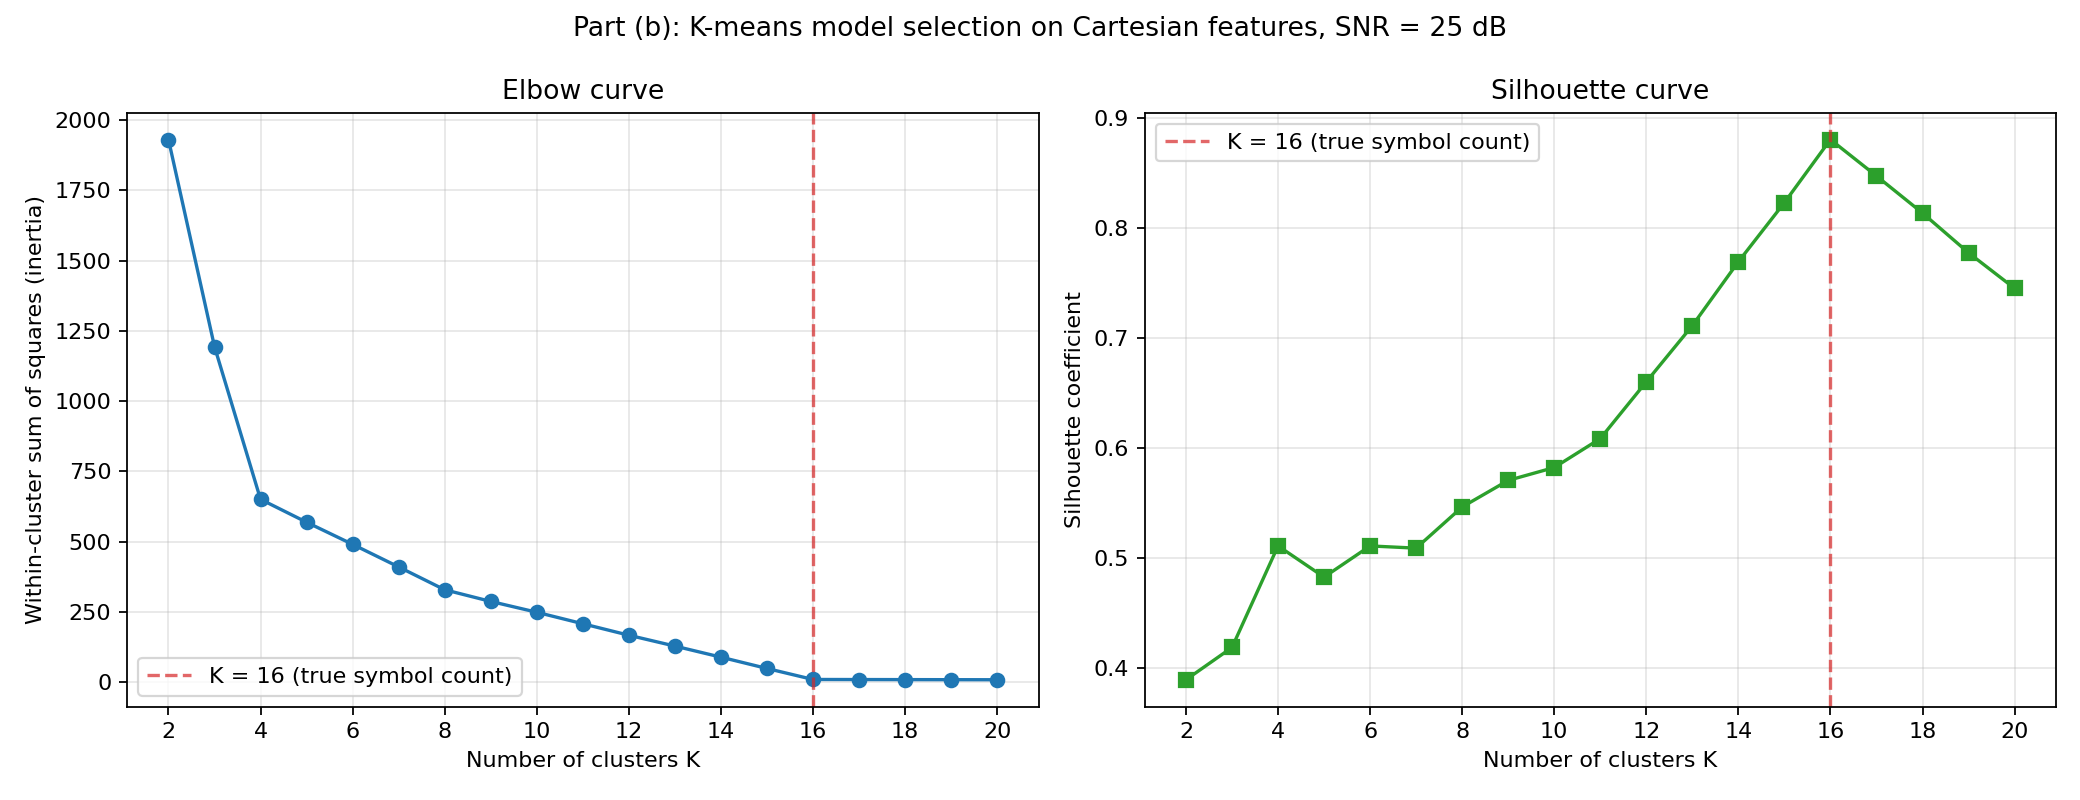
\includegraphics[width=\textwidth]{figures/partb_elbow_silhouette.png}
\caption{Inertia (left) and silhouette coefficient (right) versus the number of clusters $K$
at SNR $=25$~dB. The dashed line marks $K = 16$, the true number of constellation points.}
\label{fig:q2b1}
\end{figure}

Both metrics identify $K = 16$ unambiguously, and more sharply than a typical clustering
problem would, because this dataset genuinely has sixteen well-separated generative modes.

The inertia falls steeply and almost linearly from $K = 12$ to $K = 15$, then drops off a
cliff at $K = 16$, from 49.39 to 10.22, a 79\% reduction in a single step, and goes flat
afterwards. The interpretation is direct: below $K = 16$ at least one cluster is forced to
straddle two distinct symbol blobs, and the inertia is dominated by the inter-symbol distance
of that straddled pair. As soon as the sixteenth centroid becomes available, every cluster
collapses onto exactly one blob and the residual inertia is nothing but the AWGN variance
inside the blobs. A seventeenth centroid can only split one noise cloud in half, which buys
almost nothing.

The silhouette peaks at exactly $K = 16$ with $s = 0.8802$ and declines on both sides. The
decline above 16 is the informative half: splitting a single isotropic Gaussian blob produces
two clusters whose members are nearly as close to the neighbouring cluster as to their own,
which drives the coefficient down. Below 16 there are two smaller local bumps, at $K = 4$
($s = 0.511$) and $K = 8$ ($s = 0.546$), corresponding to the constellation's own coarse
structure --- the four quadrants and the eight half-rows of the grid --- which K-means finds
as legitimate but coarser partitions before it resolves individual symbols.

\subsubsection{Clustering with $K = 16$}

\begin{figure}[H]
\centering
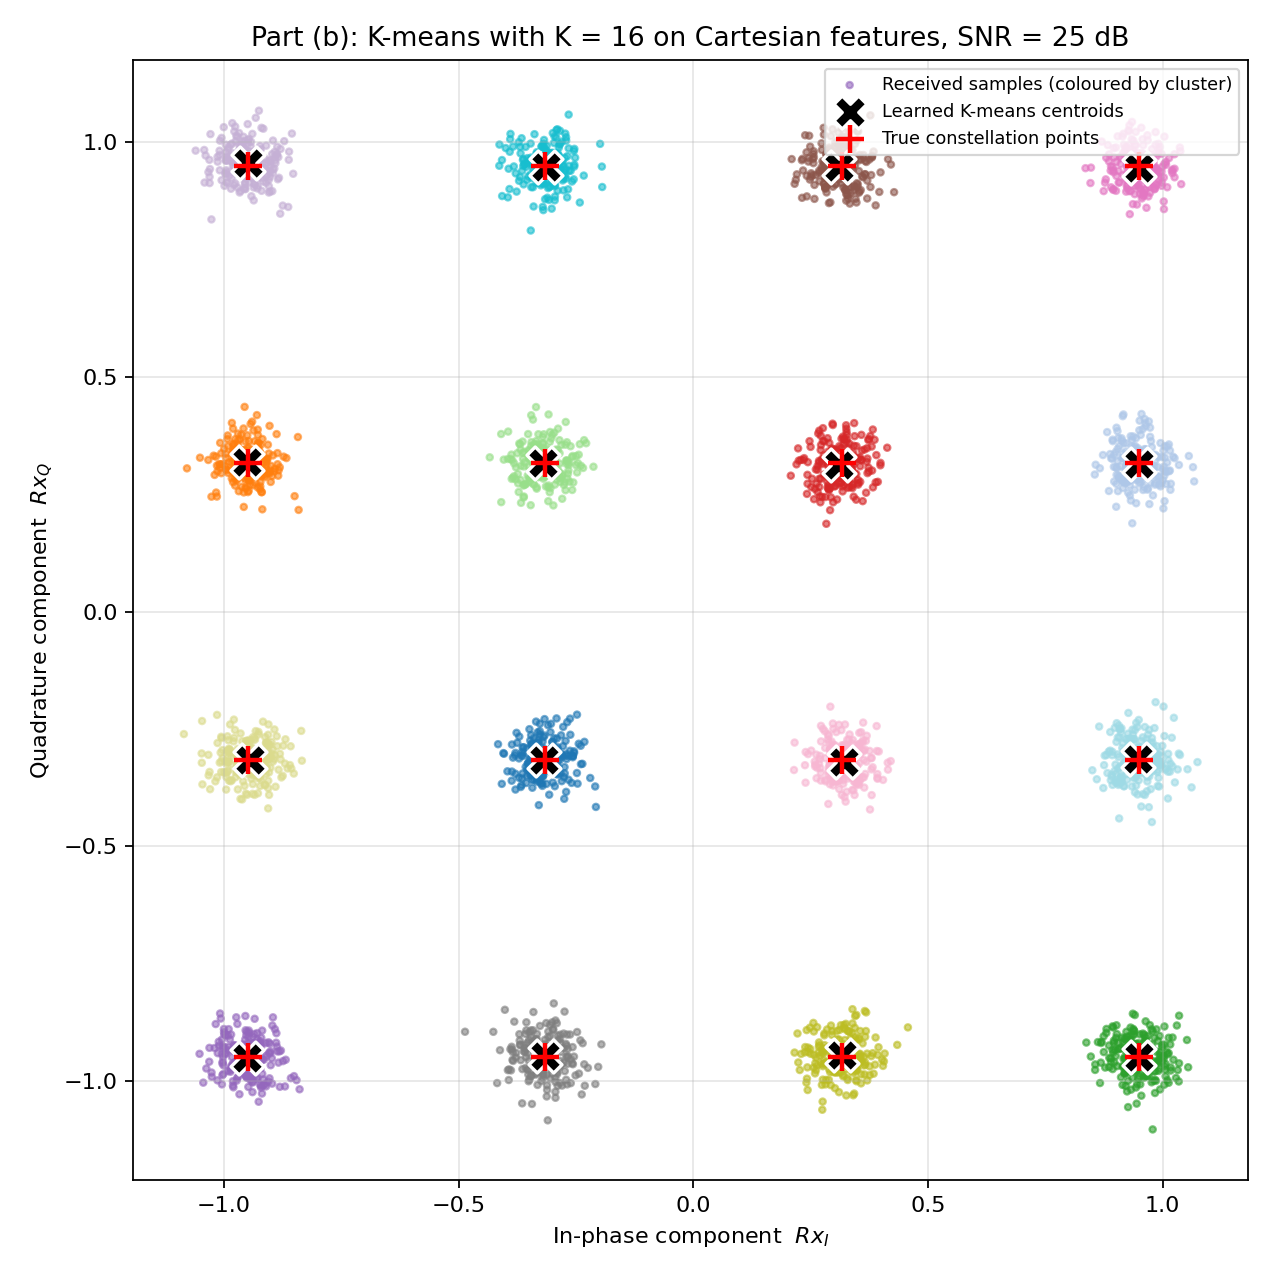
\includegraphics[width=0.72\textwidth]{figures/partb_clusters_k16_25db.png}
\caption{K-means with $K = 16$ on the Cartesian features at SNR $=25$~dB. Points are coloured
by assigned cluster, black crosses are the learned centroids, and red plus markers are the
true transmitted constellation points.}
\label{fig:q2b3}
\end{figure}

The sixteen learned centroids land on the sixteen true constellation points with an RMS
displacement of 0.0039 against a symbol spacing of 0.6325, an error of 0.6\%. Every noise
cloud is visibly compact and separated by clear empty space, and the cluster purity is
1.0000. At 25~dB, completely unsupervised K-means recovers the 16-QAM alphabet perfectly
without ever being told what a constellation is.

\subsubsection{Comparison of Feature Sets}
\label{sec:featuresets}

Cluster purity is computed as

\begin{equation}
\text{Purity} = \frac{1}{N} \sum_k \max_j \left| C_k \cap G_j \right|,
\end{equation}

where $C_k$ is a predicted cluster and $G_j$ a ground-truth symbol class: each cluster is
assigned the symbol most frequent within it, and the overall fraction of correctly assigned
samples is reported. Three representations are compared at $K = 16$: Set~1 $(x_I, x_Q)$,
Set~2 $(r, \theta)$, and Set~3 $(x_I, x_Q, r, \theta)$ with \texttt{StandardScaler} applied.
Only Set~3 is scaled, as specified.

\begin{table}[H]
\centering
\caption{Cluster purity at $K = 16$, SNR $= 25$~dB.}
\label{tab:purity25}
\begin{tabular}{lr}
\toprule
Feature set & Purity \\
\midrule
Set 1: Cartesian $(x_I, x_Q)$                      & 1.0000 \\
Set 2: Polar $(r, \theta)$                         & 1.0000 \\
Set 3: Combined $(x_I, x_Q, r, \theta)$, scaled    & 1.0000 \\
\bottomrule
\end{tabular}
\end{table}

At the required SNR all three sets are saturated. This is a real result rather than a failure
to compute: at 25~dB the clusters are separated by roughly sixteen noise standard deviations,
so even a distorted metric has enough margin to assign all 3200 samples correctly. It cannot,
however, rank the three representations. Repeating the comparison at every SNR breaks the
tie.

\begin{table}[H]
\centering
\caption{Cluster purity of the three feature sets across SNR, $K = 16$.}
\label{tab:purityall}
\begin{tabular}{crrr}
\toprule
SNR (dB) & Set 1 (Cartesian) & Set 2 (Polar) & Set 3 (Combined, scaled) \\
\midrule
 0 & \textbf{0.2547} & 0.2469 & 0.2431 \\
 5 & \textbf{0.4491} & 0.4150 & 0.4113 \\
10 & \textbf{0.7656} & 0.6966 & 0.6628 \\
15 & \textbf{0.9841} & 0.9700 & 0.9678 \\
20 & 0.9997 & 0.9994 & 0.9997 \\
25 & 1.0000 & 1.0000 & 1.0000 \\
30 & 1.0000 & 1.0000 & 1.0000 \\
\bottomrule
\end{tabular}
\end{table}

\paragraph{Which feature set produces the highest cluster purity?}
Feature Set~1, the raw Cartesian pair. It wins at every SNR where the metric is not
saturated, by as much as 10~pp at 10~dB (0.7656 against 0.6628). Set~2 is second and Set~3
last.

Set~3 finishing last is the mildly counter-intuitive part and deserves an explicit statement.
Adding $r$ and $\theta$ adds no \emph{information}, because they are a deterministic and
invertible function of $(x_I, x_Q)$. What Set~3 adds is \emph{weight}: after standardisation
all four axes carry equal variance, so the two distorted polar axes influence the distance
metric exactly as much as the two well-conditioned Cartesian ones. The distortion described
below is imported into an otherwise clean representation and dilutes it. Redundant features
are not free when the algorithm's only mechanism is a distance.

\paragraph{Why does Euclidean distance suit Cartesian coordinates but distort unweighted
polar ones?}
Cartesian is the right space because the noise lives there. The channel adds independent
zero-mean Gaussian noise of equal variance to $x_I$ and $x_Q$, so its density contours are
circles in the I/Q plane, and the maximum-likelihood detector for AWGN is the
minimum-Euclidean-distance detector whose decision regions are the Voronoi cells of the
constellation. K-means is built on the same two assumptions --- isotropic clusters of equal
spread, partitioned by Euclidean Voronoi boundaries --- so the algorithm's inductive bias
matches the physics of the channel exactly, with no modelling mismatch to pay for. On top of
that, the 16-QAM grid is uniformly spaced along both axes, so equal Euclidean distance
corresponds to equal error probability everywhere in the plane. Unsupervised K-means at
$K = 16$ is in effect blindly rediscovering the ML detector.

Polar coordinates break this in four separate ways.

\begin{enumerate}
\item \textbf{The units do not commute.} $r$ spans roughly $[0, 1.34]$ while $\theta$ spans
$[-\pi, \pi]$, a range $4.7\times$ larger. In an unweighted sum
$(\Delta r)^2 + (\Delta\theta)^2$ the phase axis silently dominates, so the algorithm
partitions mostly by angle and under-uses amplitude. Adding a squared amplitude to a squared
angle is not a physically meaningful quantity in the first place.

\item \textbf{$\Delta\theta$ is not proportional to real distance.} Two points at radius $r$
separated by $\Delta\theta$ are physically $2r\sin(\Delta\theta/2)$ apart, but the polar
metric charges them $\Delta\theta$ regardless of $r$. Phase differences are therefore
over-weighted near the origin and under-weighted far from it. For 16-QAM this is severe: the
four inner symbols sit at $r = 0.447$ and the four corner symbols at $r = 1.342$, a factor of
three, so the inner symbols have their angular separation exaggerated threefold relative to
the corners and the metric is inconsistent across the very constellation it must partition.

\item \textbf{$\theta$ is circular but the metric is not.} $\theta = +\pi$ and
$\theta = -\pi$ are the same physical direction yet maximally far apart in Euclidean terms,
so any cluster straddling the negative real axis is torn in two. At 25~dB no symbol sits
close enough to the wrap for this to matter, but at low SNR the noise pushes samples across
it.

\item \textbf{Neither polar coordinate alone separates the alphabet.} 16-QAM has only three
distinct radii --- $0.447$ for four symbols, $1.000$ for eight and $1.342$ for four --- so
amplitude alone can never resolve sixteen classes. Several symbols also share a phase
exactly, for instance $(1,1)$ and $(3,3)$ both at $\theta = \pi/4$, so phase alone cannot
either. The two must be combined with the correct relative weighting, and unweighted
Euclidean distance is not it.
\end{enumerate}

The net effect is decision boundaries that are wedges and annuli in the physical plane rather
than the square Voronoi cells the AWGN channel calls for. Set~2 still reaches purity 1.0000
at 25~dB only because the clusters are so far apart that even a badly shaped boundary
separates them; as soon as the noise grows, Set~2 falls behind Set~1 and stays behind.

%------------------------------------------------------------------------------
\subsection{Adaptive K-Means versus Fixed Template}
%------------------------------------------------------------------------------

Two demodulation strategies are compared at $K = 16$. The adaptive strategy fits a fresh
K-means model on each SNR's own Cartesian data and scores its purity there. The fixed-template
strategy fits once at 25~dB, freezes those centroids, and only predicts at every SNR.

\begin{table}[H]
\centering
\caption{Cluster purity of the two demodulation strategies, $K = 16$.}
\label{tab:q2c}
\begin{tabular}{crrr}
\toprule
SNR (dB) & Adaptive K-Means & Fixed Template & Fixed $-$ Adaptive \\
\midrule
 0 & 0.2547 & \textbf{0.2631} & $+0.0084$ \\
 5 & 0.4491 & \textbf{0.4722} & $\mathbf{+0.0231}$ \\
10 & 0.7656 & \textbf{0.7725} & $+0.0069$ \\
15 & \textbf{0.9841} & 0.9838 & $-0.0003$ \\
20 & 0.9997 & 0.9997 & $0.0000$ \\
25 & 1.0000 & 1.0000 & $0.0000$ \\
30 & 1.0000 & 1.0000 & $0.0000$ \\
\bottomrule
\end{tabular}
\end{table}

\begin{figure}[H]
\centering
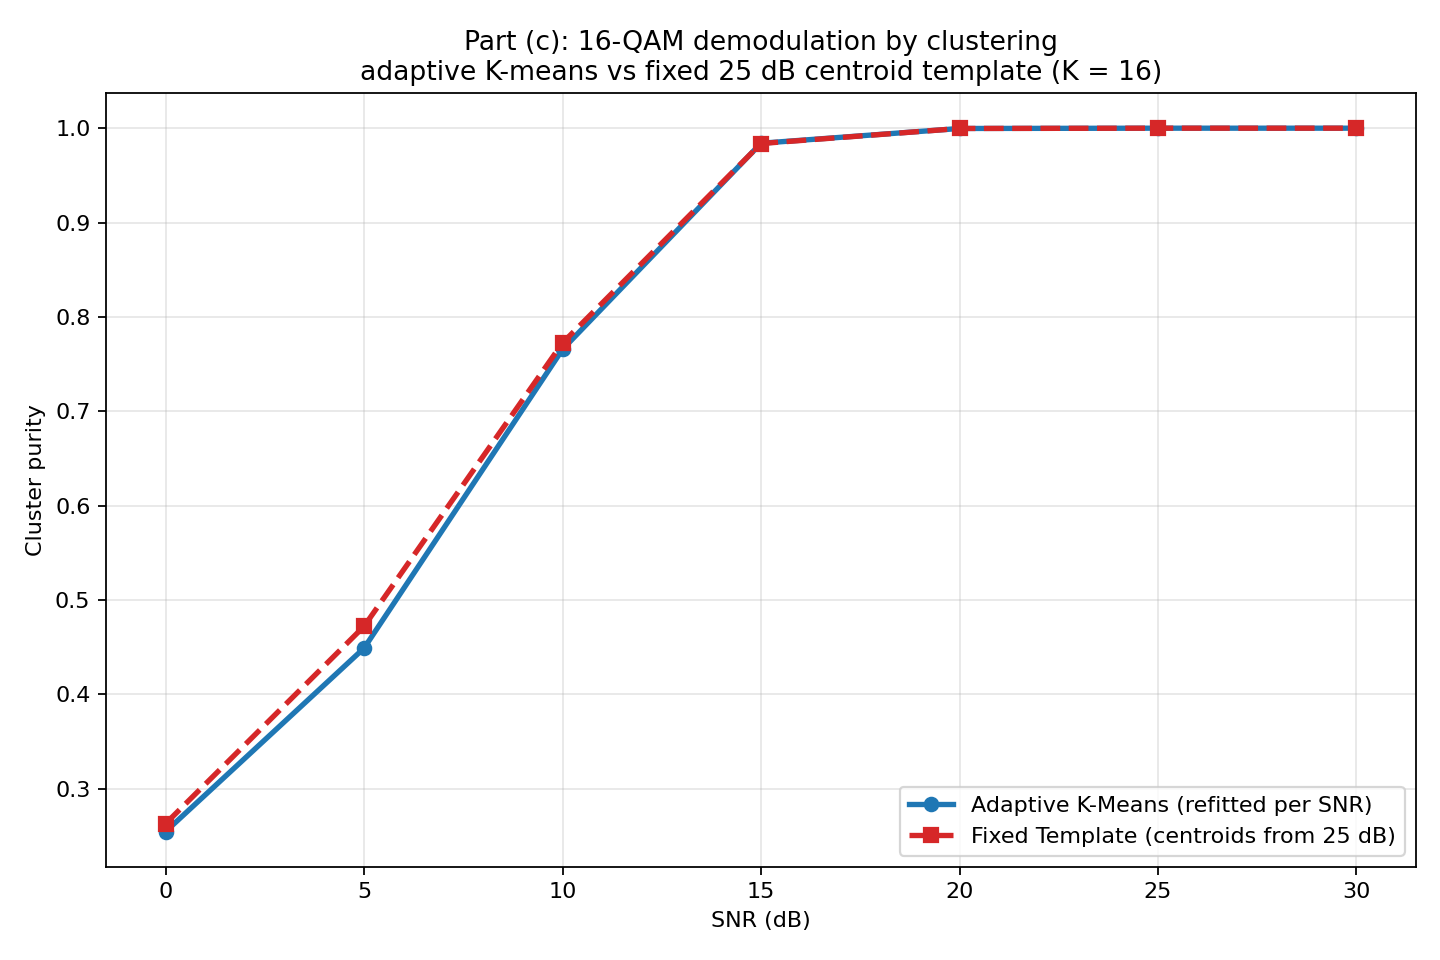
\includegraphics[width=0.85\textwidth]{figures/partc_adaptive_vs_fixed.png}
\caption{Cluster purity versus SNR for adaptive K-means and the fixed 25~dB centroid
template.}
\label{fig:q2c}
\end{figure}

\subsubsection{Discussion}

\paragraph{At high SNR, do the two curves agree, and what does that say about centroid
stability?}
They agree identically. Both reach purity 1.0000 at 25 and 30~dB and 0.9997 at 20~dB, a
single misassigned sample out of 3200, and the curves are indistinguishable above roughly
15~dB.

This indicates that the centroids are fully identifiable and stable in the low-noise regime.
Table~\ref{tab:geometry} quantifies how tightly: it reports, for the adaptive fit at each
SNR, the RMS distance from each learned centroid to its nearest true constellation point, and
the smallest distance between any two learned centroids.

\begin{table}[H]
\centering
\caption{Adaptive centroid geometry against the true constellation grid. The true
nearest-neighbour spacing is 0.6325; the fixed template's values are 0.0039 and 0.6258 by
construction and do not vary with SNR.}
\label{tab:geometry}
\begin{tabular}{crr}
\toprule
SNR (dB) & RMS error to true grid & Minimum centroid gap \\
\midrule
 0 & 0.5744 & 0.8561 \\
 5 & 0.2347 & 0.6555 \\
10 & 0.0536 & 0.5680 \\
15 & 0.0112 & 0.6046 \\
20 & 0.0062 & 0.6177 \\
25 & 0.0039 & 0.6258 \\
30 & 0.0021 & 0.6285 \\
\bottomrule
\end{tabular}
\end{table}

Above 15~dB the adaptive fit recovers the true constellation to within 1--2\% of the symbol
spacing, so refitting converges to the same sixteen points the template already holds and
changes nothing. In practice, once $\sigma / \text{spacing} < 0.2$, a receiver can learn the
constellation once and freeze it; per-SNR re-estimation is wasted computation.

\paragraph{At low SNR, which strategy achieves higher accuracy?}
The fixed template, consistently: $+0.0231$ at 5~dB, $+0.0084$ at 0~dB and $+0.0069$ at
10~dB. It wins at every SNR below 15~dB.

The margin is modest in absolute terms, which is worth stating honestly. At 0~dB both
strategies are near-useless, 0.2547 and 0.2631 against a chance floor of $1/16 = 0.0625$, so
the template is not rescuing anything; the information has already been destroyed by the
channel. What the comparison shows is that the template never makes matters worse, whereas
the adaptive fit sometimes does. The difference peaks at 5~dB, where the clusters are still
partly resolvable but no longer resolvable enough for K-means to place its own centroids
correctly.

\paragraph{Why does fitting on low-SNR samples cause centroid merging?}
At 0~dB the per-axis $\sigma$ is 0.707 while adjacent symbols are 0.6325 apart, so the noise
standard deviation exceeds the symbol spacing (Table~\ref{tab:noise}). Each of the sixteen
Gaussian blobs has a radius larger than the gap to its neighbour, and they superpose into a
single broad, roughly unimodal cloud. The density minima that once sat between symbols are
gone, so there is nothing left in the data for a density-seeking algorithm to lock onto.

K-means does not detect this. It minimises within-cluster sum of squares, so given 3200 points
drawn from one broad cloud and sixteen centroids it does the only thing its objective rewards:
it tiles the cloud into sixteen roughly equal-mass Voronoi cells, placed to balance point mass
rather than to sit on the generative modes. Table~\ref{tab:geometry} shows the consequence at
0~dB. The adaptive centroids drift an RMS 0.5744 off the true grid, which is 91\% of a full
symbol spacing --- each centroid is nearly a whole symbol away from where it belongs --- and
their minimum pairwise gap swells to 0.8561, larger than the true grid's 0.6325, because they
have spread outward to cover the noise tails, which occupy a far larger area than the
constellation itself.

The merging follows directly. If centroids migrate outward to tile the sparse but wide noise
tails, the crowded interior of the constellation is left under-served: several true symbols
end up sharing a single cluster while other clusters cover regions containing no symbol
centre at all. The majority vote inside cluster purity then credits only the most frequent
symbol in each merged cluster and counts the rest as errors, which is exactly the penalty the
metric is designed to apply.

The fixed template avoids all of this by not being fitted to the data at all. Its centroids
are pinned to the true constellation geometry, so prediction at any SNR reduces to assigning
each received sample to its nearest constellation point --- a minimum-distance detector, which
is the ML detector for AWGN. It cannot recover information the noise has destroyed, so its
purity still falls to 0.2631 at 0~dB, but it is optimal given the noise and therefore acts as
a floor that adaptive fitting can match at high SNR and can only fall below at low SNR.

%==============================================================================
\section{Conclusion}
%==============================================================================

Both questions converge on the same underlying point from opposite directions: how much a
learning algorithm should be allowed to estimate from noisy data, and how much structure
should be imposed on it in advance.

In Question~1, the five channel features split cleanly into two families. The RMS delay spread
reads the delay axis, which the generator leaves noiseless, and is therefore the strongest
single feature at every SNR, from 88.50\% at 0~dB to 98.75\% at 30~dB. Kurtosis, skewness and
the Rician $K$-factor read only the amplitude distribution across six taps and collapse to
58--60\% at 0~dB, because at that SNR the added noise is roughly eight times stronger than the
scattered taps it sits on and the LOS statistics migrate onto the NLOS ones. Combining all
five features reaches 100\% above 20~dB and gains most at 5--10~dB, where the two families
make weakly correlated errors. Training at a single SNR is safe above roughly 15~dB and
catastrophic below it, costing 31.25~pp at 0~dB, and the failure is asymmetric: a model
trained at 0~dB instead holds about 90\% across the entire range but never reaches 100\%.

In Question~2, both the elbow and the silhouette identify $K = 16$ unambiguously at 25~dB,
where unsupervised K-means recovers the constellation with an RMS centroid error of 0.6\% of
the symbol spacing and purity 1.0000. The raw Cartesian pair is the best representation
because Euclidean distance in the I/Q plane is exactly the geometry the AWGN channel imposes;
unweighted polar coordinates distort it, and adding them to the Cartesian pair only imports
that distortion. Below 15~dB the fixed 25~dB template beats adaptive refitting, because once
the per-axis noise exceeds the symbol spacing the sixteen blobs merge into one cloud and
K-means tiles it by point mass, drifting its centroids 91\% of a symbol spacing off the true
grid, while the template stays pinned to the constellation and degenerates gracefully into a
minimum-distance detector.

The common lesson is that unsupervised clustering estimates geometry from data while a
template imposes geometry that is already known. When the data are clean, the two agree and
the estimate costs nothing. When the data are noisy, estimating a structure that is already
known does not merely waste effort --- it actively injects error, because the estimator will
faithfully fit whatever noise it is handed.

\end{document}
